\cleardoublepage

\chapter{Studium przypadku: aplikacja eShop}
\label{cha:StudiumPrzypadku}

Niniejszy rozdział prezentuje studium przypadku systemu eShop -- platformy testowej zbudowanej na~potrzeby niniejszej pracy, stanowiącej jednocześnie przedmiot badań eksperymentalnych opisanych w~rozdziałach~\ref{cha:MetodologiaBadan} i~\ref{cha:AnalizaWydajnosci}. Opis stanowi rozwinięcie sekcji~\ref{sec:ProjektAplikacji}, w~której przedstawiono wyłącznie te~elementy projektu, które są~niezbędne do~interpretacji pomiarów. Umiejscowienie rozdziału po~analizie wyników jest przy tym celowe: znaczna część omawianych tu~rozstrzygnięć implementacyjnych podlega ocenie właśnie w~świetle zmierzonych wartości -- dotyczy to~w~szczególności kosztu wzorca Transactional Outbox, empirycznego uzasadnienia rozdzielenia ścieżek odczytu i~zapisu oraz mechanizmów kontrolnych potwierdzających wiarygodność wyników. Omówiona zostaje architektura systemu (sekcja~\ref{sec:ArchitekturaSystemu}), implementacja kluczowych wzorców projektowych z~rozdziału~\ref{cha:WzorceProjektowe} (sekcja~\ref{sec:ImplementacjaWzorcow}), wdrożenie i~eksploatacja w~środowisku chmurowym wraz z~uzasadnieniem przyjętego modelu infrastruktury (sekcja~\ref{sec:WdrozenieChmurowe}), konsekwencje zmierzonych zależności dla decyzji wdrożeniowych (sekcja~\ref{sec:WnioskiWdrozeniowe}) oraz walidacja rozwiązania (sekcja~\ref{sec:TestowanieWalidacja}).

% -----------------------------------------------------------------------
\section{Architektura systemu eShop}
\label{sec:ArchitekturaSystemu}
% -----------------------------------------------------------------------

System eShop inspirowany jest aplikacją referencyjną \textit{eShop} firmy Microsoft, będącą następcą projektu \textit{eShopOnContainers}~\cite{bib:MicrosoftEShop2024}, lecz stanowi autorską implementację skoncentrowaną na~porównaniu protokołów komunikacji. Architektura składa się z~trzech warstw: warstwy prezentacji w~postaci aplikacji przeglądarkowej, warstwy usług biznesowych złożonej z~mikroserwisów .NET~10 oraz warstwy infrastrukturalnej obejmującej bazy danych, pamięć podręczną, brokera komunikatów i~komponenty obserwowalności.

Cechą wyróżniającą przyjęte rozwiązanie jest podwójna rola aplikacji przeglądarkowej. Stanowi ona jednocześnie warstwę prezentacji systemu oraz klienta pomiarowego w~eksperymencie opisanym w~rozdziale~\ref{cha:MetodologiaBadan}, obsługując wszystkie trzy ścieżki komunikacji przedstawione na~rysunku~\ref{fig:SciezkiKomunikacji}.

Warstwy te~rozłożone są~na~dwie maszyny: warstwa usług wraz z~infrastrukturą pracuje na~serwerze chmurowym, natomiast aplikacja kliencka podawana jest lokalnie, na~stacji roboczej stanowiącej klienta pomiarowego. Podział ten ma~dwie konsekwencje istotne dla eksperymentu. Pierwszą jest to, że~pobranie zasobów statycznych aplikacji odbywa się poza mierzoną ścieżką: pomiar rozpoczyna się od~interakcji użytkownika w~już~załadowanej stronie, co~omówiono w~sekcji~\ref{subsec:PomiarWPrzegladarce}. Drugą jest to, że~żądania kierowane do~usług są~żądaniami międzydomenowymi, przez co wymagają obsługi mechanizmu CORS zarówno w~serwerze pośredniczącym, jak i~w~usługach; konfiguracja ta~stanowi zatem nieodłączny element badanej ścieżki, nie zaś uproszczenie środowiska testowego. Rozwiązanie to~zapewnia, że~mierzona jest ta~sama ścieżka wykonania, która obsługuje rzeczywistego użytkownika, wraz z~deserializacją w~silniku JavaScript, narzutem biblioteki klienckiej oraz aktualizacją drzewa dokumentu.

\subsection{Warstwa usług biznesowych}
\label{subsec:WarstwaBiznesowa}

System realizuje podział na~dwa mikroserwisy zgodnie z~zasadą \textit{Bounded Context}~\cite{bib:Evans2003}:

\begin{itemize}
    \item \textbf{ProductService} (kontekst: katalog produktów) -- odpowiada za~operacje odczytu katalogu, implementuje wzorzec Cache-Aside, udostępnia procedurę strumieniowania gRPC oraz punkt końcowy izolujący narzut protokołu. Dane przechowywane w~dedykowanej bazie \texttt{eshop\_products} obejmują 2000~produktów rozłożonych na~dziesięć kategorii o~nierównomiernej liczności.
    \item \textbf{OrderService} (kontekst: proces zamówień) -- odpowiada za~tworzenie zamówień, implementuje wzorce Transactional Outbox oraz Saga. Dane przechowywane w~dedykowanej bazie \texttt{eshop\_orders}.
\end{itemize}

Każdy mikroserwis jest autonomiczną jednostką wdrożeniową z~własnym obrazem kontenera, konfiguracją połączeń oraz migracjami bazy danych realizowanymi w~podejściu Code-First.

Istotną cechą przyjętego projektu jest całkowity brak zależności pomiędzy obiema usługami: nie występują ani synchroniczne wywołania, ani wymiana komunikatów pomiędzy \texttt{ProductService} a~\texttt{OrderService}. Decyzja ta~wynika bezpośrednio z~celu badawczego: przedmiotem pomiaru jest komunikacja na~granicy klient--usługa, a~nie orkiestracja procesu obejmującego wiele usług. Wprowadzenie zależności międzyusługowej wnosiłoby do~pomiarów opóźnienie drugiej usługi, utrudniając izolację narzutu samego protokołu. Konsekwencją takiego podziału jest pełna niezależność wdrożeniowa obu komponentów oraz brak sprzężenia temporalnego, rozumianego jako wymóg jednoczesnej dostępności współpracujących usług~\cite{bib:Newman2021}.

Broker komunikatów RabbitMQ obsługuje natomiast przepływ zdarzeń wewnątrz \texttt{OrderService}: zdarzenie \texttt{OrderCreated} publikowane jest przez mechanizm Outbox, a~następnie odbierane przez maszynę stanów Sagi działającą w~tym samym procesie. Rozwiązanie to~odwzorowuje pełny łańcuch przetwarzania asynchronicznego, wraz z~jego kosztem wydajnościowym uwzględnionym w~pomiarach scenariuszy zapisu, bez wprowadzania zależności pomiędzy mikroserwisami.

\subsection{Skalowanie zbioru danych inicjalizacyjnych}
\label{subsec:ZasiewDanych}

Liczba produktów inicjalizacyjnych stanowi parametr o~bezpośrednim znaczeniu badawczym, ponieważ wyznacza górną granicę rozmiaru odpowiedzi, jaki można objąć pomiarem. Pierwotnie zbiór ten liczył 500~pozycji zapisanych mechanizmem \texttt{HasData} Entity Framework Core, który umieszcza dane w~treści migracji.

Rozszerzenie zbioru do~2000~pozycji zrealizowano jednak odmiennie: przez uzupełnienie wykonywane w~czasie uruchamiania usługi, po~zastosowaniu migracji. Powód jest praktyczny: mechanizm \texttt{HasData} zapisuje zawartość jako literalne tablice wartości zarówno w~pliku migracji, jak i~w~obrazie modelu, przez co zasiew kilku tysięcy wierszy prowadziłby do~wygenerowania plików o~rozmiarze wielu megabajtów, wydłużając kompilację oraz każde uruchomienie usługi. Procedura uzupełniająca jest idempotentna: porównuje liczbę istniejących wierszy z~wartością docelową i~wstawia wyłącznie brakujące, dzięki czemu ponowne uruchomienie kontenera nie powoduje duplikacji danych. Wartość docelowa jest przy tym konfigurowalna, co~pozwala dostosować zakres badania bez modyfikacji kodu.

\subsection{Podejście Contract-First}
\label{subsec:ContractFirst}

Kontrakty usług gRPC definiowane są~w~plikach Protocol Buffers, stanowiących jedyne źródło prawdy (ang.\ \textit{single source of truth}) dla interfejsów systemowych. Na~ich podstawie generowany jest kod zarówno po~stronie serwera (C\#, pakiet \texttt{Grpc.Tools}), jak i~klienta (TypeScript, narzędzia \texttt{@bufbuild/protoc-gen-es} oraz \texttt{@connectrpc/protoc-gen-connect-es}).

\begin{lstlisting}[
  language={},
  breaklines=true,
  caption={Definicja usługi ProductService w~Protocol Buffers},
  label=lst:ProductProto
]
syntax = "proto3";
package product;

service ProductService {
  rpc ListProducts (ListProductsRequest) returns (ListProductsResponse);
  rpc GetProduct (GetProductRequest) returns (Product);
  rpc CreateProduct (CreateProductRequest) returns (Product);
  rpc StreamProducts (StreamProductsRequest) returns (stream Product);
  rpc EchoProducts (EchoProductsRequest) returns (ListProductsResponse);
}

message Product {
  string id = 1;
  string name = 2;
  string description = 3;
  double price = 4;
  string category_id = 5;
  int32 stock = 6;
}
\end{lstlisting}

Podejście Contract-First zapewnia spójność typów na~granicy systemu i~przenosi wykrywanie niekompatybilnych zmian z~czasu wykonania na~etap kompilacji. Wartość tego mechanizmu potwierdziła się w~trakcie realizacji pracy: po~dodaniu do~kontraktu procedury \texttt{EchoProducts} kod klienta wymagał ponownego wygenerowania, a~odwołanie do~niewygenerowanych jeszcze typów komunikatów uniemożliwiło kompilację aplikacji frontendowej. Zakres tej ochrony jest przy tym ograniczony do~struktur danych: jak omówiono w~sekcji~\ref{subsec:IntegracjaAngular}, referencja do~klienta usługi zadeklarowana jest w~aplikacji jako \texttt{any}, przez co nazwy samych procedur nie podlegają weryfikacji na~etapie kompilacji.

\subsection{Topologia Docker Compose}
\label{subsec:DockerCompose}

Cały system uruchamiany jest za~pomocą Docker Compose, orkiestrującego dziewięć kontenerów z~grafem zależności opartym na~kontrolach zdrowia (ang.\ \textit{health checks}). Tabela~\ref{tab:DockerServices} przedstawia limity zasobów przydzielone poszczególnym kontenerom w~konfiguracji wdrożeniowej.

\begin{table}[htb]
\centering
\footnotesize
\caption{Limity zasobów kontenerów w~konfiguracji wdrożeniowej systemu eShop}
\label{tab:DockerServices}
\begin{tabular}{|l|l|c|c|}
\hline
\textbf{Kontener} & \textbf{Obraz} & \textbf{Limit CPU} & \textbf{Limit RAM} \\
\hline
product-service & obraz własny (.NET~10) & 4,0 & 3\,GB \\
order-service   & obraz własny (.NET~10) & 4,0 & 3\,GB \\
envoy           & envoyproxy/envoy:v1.29-latest & 4,0 & 1\,GB \\
postgres        & postgres:17-alpine & 4,0 & 4\,GB \\
redis           & redis:7.2-alpine & 1,0 & 512\,MB \\
rabbitmq        & rabbitmq:3.13-management-alpine & 2,0 & 1\,GB \\
jaeger          & jaegertracing/all-in-one:1.56 & 1,0 & 512\,MB \\
prometheus      & prom/prometheus:v2.51.2 & 1,0 & 512\,MB \\
grafana         & grafana/grafana:10.4.2 & 1,0 & 512\,MB \\
\hline
\end{tabular}
\end{table}

Suma limitów przekracza liczbę rdzeni dostępnych na~serwerze, co~stanowi świadome nadmiarowe przydzielenie zasobów. Limity pełnią w~tym zastosowaniu funkcję zabezpieczenia przed monopolizacją hosta przez pojedynczy kontener, nie zaś mechanizmu rezerwacji. Przy zaobserwowanym poziomie obciążenia nie stanowiły one czynnika ograniczającego, czego potwierdzeniem jest wykazane w~sekcji~\ref{sec:GranicaNarzedzia} umiejscowienie wąskiego gardła po~stronie klienta.

% -----------------------------------------------------------------------
\section{Implementacja wybranych wzorców}
\label{sec:ImplementacjaWzorcow}
% -----------------------------------------------------------------------

System eShop demonstruje praktyczne zastosowanie wzorców opisanych w~rozdziale~\ref{cha:WzorceProjektowe}: Cache-Aside, Transactional Outbox, Saga oraz strumieniowania serwerowego.

\subsection{Wzorzec Cache-Aside w~ProductService}
\label{subsec:CacheAsideImpl}

Implementacja wzorca Cache-Aside, omówionego w~sekcji~\ref{sec:CacheAside}, wykorzystuje interfejs \texttt{IDistributedCache} z~dostawcą Redis oraz klucz złożony z~parametrów zapytania. Listing~\ref{lst:CacheAside} przedstawia obsługę trafienia i~chybienia w~usłudze gRPC.

\begin{lstlisting}[
  language={[Sharp]C},
  breaklines=true,
  caption={Implementacja wzorca Cache-Aside w~ProductGrpcService},
  label=lst:CacheAside
]
public override async Task<ListProductsResponse> ListProducts(
    ListProductsRequest request, ServerCallContext context)
{
    bool bypassCache = context.RequestHeaders
        .Get("x-bypass-cache") != null;
    string cacheKey = $"grpcpb_products_{request.CategoryId}"
                    + $"_{page}_{pageSize}";

    if (!bypassCache)
    {
        // Cached as protobuf bytes: a single binary parse on a hit.
        var cached = await cache.GetAsync(cacheKey,
            context.CancellationToken);
        if (cached is { Length: > 0 })
        {
            try { return ListProductsResponse.Parser.ParseFrom(cached); }
            catch (InvalidProtocolBufferException) { /* fall through */ }
        }
    }

    // Cache miss - query PostgreSQL
    var entities = await query.Skip((page - 1) * pageSize).Take(pageSize)
        .ToListAsync(context.CancellationToken);

    var response = new ListProductsResponse { TotalCount = totalCount };
    response.Products.AddRange(entities.Select(e => e.ToProto()));

    await cache.SetAsync(cacheKey, response.ToByteArray(),
        new DistributedCacheEntryOptions {
            AbsoluteExpirationRelativeToNow = TimeSpan.FromMinutes(5)
        }, context.CancellationToken);

    return response;
}
\end{lstlisting}

Przedstawiona postać implementacji jest wynikiem korekty wprowadzonej na~etapie przygotowania eksperymentu i~zasługuje na~komentarz, ponieważ ilustruje klasę błędów trudnych do~wykrycia w~badaniach porównawczych. W~wersji pierwotnej usługa gRPC przechowywała w~pamięci podręcznej reprezentację JSON, którą przy każdym trafieniu deserializowała, aby następnie ponownie zserializować wiadomość do~formatu Protocol Buffers. Punkt końcowy REST zapisywał natomiast gotowy dokument JSON i~przy trafieniu zwracał go~bez żadnej serializacji. Obie ścieżki wykonywały zatem różną ilość pracy, z~przyczyn niezwiązanych z~badanymi protokołami, co~systematycznie obciążało wyniki wariantów binarnych.

Przechowywanie binarnej postaci wiadomości redukuje obsługę trafienia do~jednorazowej analizy składniowej danych binarnych. Resztkowa asymetria pozostaje, ponieważ ścieżka REST nadal nie wykonuje żadnej serializacji, lecz działa ona na~niekorzyść wariantów gRPC-Web, a~zatem nie może być źródłem wykazanej w~rozdziale~\ref{cha:AnalizaWydajnosci} przewagi tych wariantów. Zagadnienie omówiono w~sekcji~\ref{sec:Ograniczenia}.

Nagłówek \texttt{X-Bypass-Cache} umożliwia programowe wymuszenie zapytania do~bazy danych, co~wykorzystano w~eksperymencie do~realizacji scenariuszy z~zimną pamięcią podręczną (sekcja~\ref{subsec:TestyObciazeniowe}). Odrębne przestrzenie nazw kluczy dla obu protokołów zapobiegają próbie interpretacji dokumentu zapisanego przez jedną ścieżkę przez drugą.

\subsection{Wzorzec Transactional Outbox w~OrderService}
\label{subsec:OutboxImpl}

Wzorzec Transactional Outbox gwarantuje atomowość zapisu encji biznesowej oraz publikacji zdarzenia domenowego. W~systemie eShop realizowany jest przez pakiet MassTransit z~integracją EF~Core~\cite{bib:MassTransit}.

\begin{lstlisting}[
  language={[Sharp]C},
  breaklines=true,
  caption={Konfiguracja wzorca Transactional Outbox w~OrderService},
  label=lst:OutboxConfig
]
builder.Services.AddMassTransit(x =>
{
    // Outbox in EF Core - messages persisted in the OutboxMessage table
    x.AddEntityFrameworkOutbox<OrdersDbContext>(o =>
    {
        o.UsePostgres();
        o.UseBusOutbox(); // separate delivery process publishes to RabbitMQ
    });

    x.AddSagaStateMachine<OrderProcessingSaga, OrderSagaState>()
        .EntityFrameworkRepository(r =>
        {
            r.ExistingDbContext<OrdersDbContext>();
            r.UsePostgres();
        });

    x.UsingRabbitMq((context, cfg) =>
    {
        cfg.Host(builder.Configuration.GetConnectionString("RabbitMQ"));
        cfg.ConfigureEndpoints(context);
    });
});
\end{lstlisting}

Mechanizm działa dwuetapowo. W~pierwszym etapie punkt końcowy zapisuje encję zamówienia oraz komunikat \texttt{OrderCreated} w~jednej transakcji bazodanowej. W~drugim odrębny wątek dostarczający odczytuje niedostarczone komunikaty i~publikuje je~do~brokera. Gwarancja dostarczenia co~najmniej jednokrotnego eliminuje scenariusz, w~którym zamówienie zostaje zapisane, lecz zdarzenie nie dociera do~Sagi.

\begin{lstlisting}[
  language={[Sharp]C},
  breaklines=true,
  caption={Endpoint tworzenia zamówienia z~publikacją zdarzenia przez Outbox},
  label=lst:OrderEndpoint
]
app.MapPost("/api/orders", async (OrdersDbContext db,
    IPublishEndpoint publishEndpoint, CreateOrderDto dto) =>
{
    var entity = new OrderEntity
    {
        CustomerId = dto.CustomerId,
        TotalPrice = dto.Items.Sum(i => i.UnitPrice * i.Quantity),
        Items = dto.Items.Select(i => new OrderItemEntity
        {
            ProductId = i.ProductId,
            ProductName = i.ProductName,
            Quantity = i.Quantity,
            UnitPrice = i.UnitPrice,
        }).ToList(),
    };
    db.Orders.Add(entity);

    // Published via Outbox - persisted atomically with the entity
    await publishEndpoint.Publish(new OrderCreated
    {
        OrderId = entity.Id,
        CustomerId = entity.CustomerId,
        TotalPrice = (decimal)entity.TotalPrice,
        CreatedAt = entity.CreatedAt
    });

    await db.SaveChangesAsync(); // single transaction: entity + outbox msg
    return Results.Created($"/api/orders/{entity.Id}", entity.ToProto());
});
\end{lstlisting}

Koszt wydajnościowy tego rozwiązania zmierzono w~scenariuszach zapisu (sekcja~\ref{sec:AnalizaOrders}). Stanowi on~stały składnik rzędu 60--70~ms ponad opóźnienie sieciowe, niezależny od~wybranego protokołu komunikacji.

\subsection{Maszyna stanów Saga}
\label{subsec:SagaImpl}

Wzorzec Saga orkiestruje wieloetapowy proces realizacji zamówienia za~pomocą maszyny stanów MassTransit.

\begin{lstlisting}[
  language={[Sharp]C},
  breaklines=true,
  caption={Implementacja maszyny stanów OrderProcessingSaga},
  label=lst:SagaImpl
]
public class OrderProcessingSaga : MassTransitStateMachine<OrderSagaState>
{
    public State AwaitingPayment { get; private set; } = null!;
    public State Completed { get; private set; } = null!;
    public State Cancelled { get; private set; } = null!;

    public Event<OrderCreated> OrderCreated { get; private set; } = null!;
    public Event<PaymentReceived> PaymentReceived { get; private set; } = null!;
    public Event<OrderCompleted> OrderCompleted { get; private set; } = null!;
    public Event<OrderCancelled> OrderCancelled { get; private set; } = null!;

    public OrderProcessingSaga()
    {
        InstanceState(x => x.CurrentState);

        Event(() => OrderCreated,
            x => x.CorrelateById(ctx => ctx.Message.OrderId));
        Event(() => PaymentReceived,
            x => x.CorrelateById(ctx => ctx.Message.OrderId));
        Event(() => OrderCompleted,
            x => x.CorrelateById(ctx => ctx.Message.OrderId));
        Event(() => OrderCancelled,
            x => x.CorrelateById(ctx => ctx.Message.OrderId));

        Initially(
            When(OrderCreated)
                .Then(ctx =>
                {
                    ctx.Saga.CustomerId = ctx.Message.CustomerId;
                    ctx.Saga.TotalAmount = ctx.Message.TotalPrice;
                    ctx.Saga.CreatedAt = ctx.Message.CreatedAt;
                })
                .TransitionTo(AwaitingPayment)
        );

        During(AwaitingPayment,
            When(PaymentReceived).TransitionTo(Completed),
            When(OrderCancelled).TransitionTo(Cancelled)
        );

        During(Completed,
            When(OrderCompleted).Finalize()
        );

        SetCompletedWhenFinalized();
    }
}
\end{lstlisting}

Maszyna stanów definiuje przejście ze~stanu początkowego \texttt{Initial} do~stanu \texttt{AwaitingPayment}, a~następnie, zależnie od~przebiegu procesu, do~stanu \texttt{Completed} albo \texttt{Cancelled}, wraz z~zakończeniem instancji po~zdarzeniu \texttt{OrderCompleted}. Stan instancji utrwalany jest w~tabeli \texttt{OrderSagas} za~pośrednictwem repozytorium EF~Core, co~zapewnia odporność na~awarie procesu: po~restarcie usługi Saga wznawia przetwarzanie od~ostatniego zapisanego stanu.

Zakres faktycznego wykorzystania tej maszyny w~zrealizowanym systemie jest przy tym węższy od~jej definicji, ponieważ jedynym publikowanym zdarzeniem jest \texttt{OrderCreated}. Instancja Sagi powstaje zatem, koreluje zdarzenie początkowe i~pozostaje w~stanie \texttt{AwaitingPayment}, natomiast dalsze przejścia stanowią kod nieosiągalny. Zagadnienie to~wraz z~jego konsekwencjami dla interpretacji pomiarów omówiono w~rozdziale~\ref{cha:WzorceProjektowe}.

\subsection{Strumieniowanie serwerowe}
\label{subsec:StreamingImpl}

\texttt{ProductService} implementuje strumieniowanie po~stronie serwera z~wykorzystaniem interfejsu \texttt{IAsyncEnumerable} oraz metody \texttt{AsAsyncEnumerable} EF~Core, co~umożliwia przesyłanie danych bez buforowania pełnego zbioru wyników w~pamięci.

\begin{lstlisting}[
  language={[Sharp]C},
  breaklines=true,
  caption={Strumieniowanie gRPC z~użyciem IAsyncEnumerable},
  label=lst:StreamImpl
]
public override async Task StreamProducts(StreamProductsRequest request,
    IServerStreamWriter<Product> responseStream, ServerCallContext context)
{
    var query = db.Products.AsNoTracking().AsQueryable();
    if (!string.IsNullOrEmpty(request.CategoryId))
        query = query.Where(p => p.CategoryId == request.CategoryId);

    await foreach (var entity in query.AsAsyncEnumerable()
        .WithCancellation(context.CancellationToken))
    {
        await responseStream.WriteAsync(entity.ToProto());
    }
}
\end{lstlisting}

Podejście to~łączy natywne mechanizmy platformy .NET z~protokołem gRPC, realizując wzorzec \textit{reactive pull}, w~którym klient steruje tempem odbioru danych poprzez mechanizm kontroli przepływu protokołu HTTP/2~\cite{bib:RFC9113}. Poprawność implementacji zweryfikowano funkcjonalnie w~aplikacji przeglądarkowej, korzystającej z~przyrostowego odbioru wiadomości; mechanizm ten nie był natomiast przedmiotem pomiarów wydajnościowych, co~wynika z~zakresu eksperymentu określonego w~sekcji~\ref{sec:CeleHipotezy}.

% -----------------------------------------------------------------------
\section{Wdrożenie i~eksploatacja w~środowisku chmurowym}
\label{sec:WdrozenieChmurowe}
% -----------------------------------------------------------------------

System testowy wdrożono w~publicznej chmurze obliczeniowej, w~modelu infrastruktury jako usługi (ang.\ \textit{infrastructure as a~service}). Niniejsza sekcja przedstawia przyjęty model wdrożenia wraz z~jego uzasadnieniem, przebieg wdrożenia, warstwę obserwowalności oraz automatyzację budowania. Rozstrzygnięcia omówione poniżej wynikają w~znacznej mierze z~wymagań eksperymentu, nie wyłącznie z~praktyki eksploatacyjnej, i~w~tym kontekście zostały przedstawione.

\subsection{Uzasadnienie przyjętego modelu wdrożenia}
\label{subsec:ModelWdrozenia}

Wszystkie komponenty systemu uruchomiono jako kontenery na~pojedynczej instancji maszyny wirtualnej, zarządzane narzędziem Docker Compose w~konfiguracji przedstawionej w~tabeli~\ref{tab:DockerServices}. Rozwiązanie alternatywne, to~jest wdrożenie w~klastrze zarządzanym platformą Kubernetes wraz z~automatycznym skalowaniem poziomym, rozważono i~odrzucono ze~względu na~wymagania pomiarowe. Uzasadnienie tej decyzji wymaga przedstawienia, ponieważ dotyczy ona podstawowego rozstrzygnięcia architektonicznego części praktycznej.

Przesłanka pierwsza dotyczy rozdzielczości pomiaru. Warstwa orkiestracji wprowadza własny mechanizm rozmieszczania obciążenia oraz sieć nakładkową, w~której ruch pomiędzy komponentami podlega dodatkowym przekształceniom adresowym, a~w~konfiguracji wielowęzłowej także dodatkowym skokom sieciowym. Różnice pomiędzy badanymi protokołami wynoszą, jak wykazano w~rozdziale~\ref{cha:AnalizaWydajnosci}, jeden obieg pakietu przy dużych ładunkach, natomiast od~jednej do~pięciu milisekund w~zakresie ładunków małych. Składniki czasu wnoszone przez warstwę orkiestracji byłyby względem tych wielkości nieznane i~zmienne, co~uniemożliwiłoby przypisanie zmierzonej różnicy badanemu czynnikowi.

Przesłanka druga dotyczy stałości warunków. Mechanizmy automatycznego skalowania oraz ponownego rozmieszczania kontenerów zmieniają liczbę i~lokalizację instancji w~czasie działania systemu, natomiast macierz badawcza wykonywana jest w~jednym ciągu trwającym 69,7~minuty (sekcja~\ref{subsec:WymiaryMacierzy}). Topologia stała nie stanowi w~tych warunkach uproszczenia, lecz warunek powtarzalności pomiaru.

Przyjęty model nie jest zatem podyktowany wygodą, lecz celem badawczym: przedmiotem pomiaru jest narzut protokołu komunikacji, nie właściwości platformy orkiestracji. Wdrożenie systemu w~klastrze wraz z~pomiarem wpływu liczby replik na~czas odpowiedzi wskazano jako kierunek dalszych badań.

\subsection{Infrastruktura utrzymywana samodzielnie a~usługi zarządzane}
\label{subsec:SelfHosted}

Bazę danych PostgreSQL, pamięć podręczną Redis oraz brokera komunikatów RabbitMQ uruchomiono jako kontenery na~tej~samej maszynie, mimo że~każdy z~tych komponentów dostępny jest u~dostawców chmurowych w~postaci usługi zarządzanej. Wybór ten wynika z~trzech przesłanek o~charakterze metodycznym.

Pierwszą jest kontrola nad~ścieżką sieciową. Usługa zarządzana udostępniana jest pod~adresem, za~którym znajduje się nieujawniana liczba elementów pośredniczących, a~wnoszone przez nią~opóźnienie stanowi składnik nieznany i~niepodlegający pomiarowi z~poziomu aplikacji. W~scenariuszach zapisu, w~których czas odpowiedzi zdominowany jest przez transakcję bazodanową, składnik taki obciążałby wynik w~sposób nieudokumentowany.

Drugą jest jawne przypięcie wersji. Wersje obrazów kontenerów określone są~w~konfiguracji wdrożeniowej wprost, natomiast usługi zarządzane podlegają aktualizacjom realizowanym przez dostawcę, w~tym potencjalnie w~trakcie okna pomiarowego. Powtarzalność eksperymentu wymaga, aby wersja każdego komponentu była znana i~niezmienna.

Trzecią jest możliwość ingerencji w~stan komponentów. Scenariusze z~zimną pamięcią podręczną oraz zmiana zbioru danych inicjalizacyjnych wymagały unieważniania zawartości pamięci podręcznej i~ponownego zasiewu bazy, a~zatem dostępu administracyjnego, który usługi zarządzane udostępniają w~zakresie ograniczonym.

Rozwiązanie to~ma~przy tym wyraźny koszt: odpowiedzialność za~kopie zapasowe, aktualizacje bezpieczeństwa oraz dostępność pozostaje po~stronie zespołu utrzymującego system, a~pojedyncza maszyna nie zapewnia odporności na~awarię sprzętową. W~zastosowaniu produkcyjnym rachunek ten wypada zwykle na~korzyść usług zarządzanych. W~zastosowaniu badawczym rozstrzygająca jest natomiast kontrola nad~warunkami pomiaru, co~stanowi jednocześnie ograniczenie przenoszalności wyników: opisują one system zestawiony w~przedstawiony sposób, nie dowolną konfigurację chmurową.

\subsection{Proces wdrożenia}
\label{subsec:Deployment}

System wdrożono na~serwerze chmury Hetzner Cloud o~ośmiu rdzeniach wirtualnych i~16~GB pamięci, z~wykorzystaniem Docker Compose w~konfiguracji wdrożeniowej. Proces wdrożenia obejmuje konfigurację serwera wraz z~wygenerowaniem certyfikatów TLS, uruchomienie stosu z~oczekiwaniem na~kontrole zdrowia wszystkich kontenerów, weryfikację punktów końcowych gotowości każdego mikroserwisu oraz wykonanie automatycznych migracji bazy danych przy starcie usług.

Konfiguracja wdrożeniowa nie obejmuje kompresji ciała odpowiedzi, ani w~usługach, ani w~serwerze pośredniczącym; pozostawiono w~tym zakresie domyślne ustawienia platformy. Decyzja ta~ma~znaczenie dla zakresu wniosków i~omówiono ją~w~sekcji~\ref{subsec:Kompresja}.

Graf zależności Docker Compose zapewnia prawidłową kolejność uruchamiania: PostgreSQL i~Redis muszą osiągnąć stan zdrowy przed startem mikroserwisów, a~mikroserwisy -- przed startem serwera pośredniczącego. Mechanizm ten eliminuje błędy wynikające z~przedwczesnych prób połączenia z~niedostępnymi usługami. Podstawą kontroli stanu są~punkty końcowe \texttt{/healthz/live} oraz \texttt{/healthz/ready}, udostępniane przez wbudowany w~ASP.NET Core mechanizm kontroli zdrowia~\cite{bib:MicrosoftDocs2024}.

W~trakcie wdrażania zmian wprowadzonych na~potrzeby eksperymentu ujawniła się zależność warta odnotowania. Pamięć podręczna Redis, z~czasem życia wpisu równym pięciu minutom, przechowywała dokumenty odpowiadające poprzedniemu zbiorowi danych, a~bezpośrednio po~wdrożeniu system raportował w~konsekwencji stan sprzed zmiany. Obserwacja ta~prowadzi do~wniosku o~charakterze operacyjnym: po~każdej modyfikacji wpływającej na~kształt odpowiedzi konieczne jest unieważnienie pamięci podręcznej przed rozpoczęciem pomiarów. W~przeciwnym razie eksperyment mierzyłby stan poprzedni, bez żadnego widocznego objawu błędu.

\subsection{Obserwowalność i~śledzenie rozproszone}
\label{subsec:Observability}

System integruje trzy filary obserwowalności zgodnie ze~standardem OpenTelemetry~\cite{bib:OpenTelemetry2024}:

\begin{itemize}
    \item \textbf{Metryki} -- eksportowane do~Prometheusa przez dedykowany punkt końcowy. Obejmują czas odpowiedzi, liczbę aktywnych połączeń oraz metryki środowiska uruchomieniowego .NET: przebiegi odśmiecania pamięci, stan puli wątków i~wolumen alokacji.
    \item \textbf{Ślady} (ang.\ \textit{traces}) -- eksportowane do~Jaegera protokołem OTLP. Instrumentacja obejmuje ASP.NET Core wraz z~obsługą żądań gRPC, EF~Core oraz MassTransit.
    \item \textbf{Pulpity wizualizacyjne} -- Grafana z~automatycznie wdrażaną konfiguracją źródeł danych i~definicji pulpitów.
\end{itemize}

Pulpity Grafany wdrażane są~wraz z~całym stosem, w~postaci definicji przechowywanych w~repozytorium i~wczytywanych przy starcie kontenera. Dzięki temu warstwa wizualizacji odtwarzana jest automatycznie na~każdym środowisku, bez ręcznej konfiguracji. Pierwszy z~pulpitów (rysunek~\ref{fig:GrafanaHttp}) obejmuje charakterystykę warstwy HTTP obu mikroserwisów: liczbę żądań na~sekundę oraz percentyle czasu obsługi żądania mierzone po~stronie serwera. Drugi (rysunek~\ref{fig:GrafanaRuntime}) przedstawia rozbicie liczby żądań na~poszczególne trasy oraz metryki środowiska uruchomieniowego .NET: wolumen alokacji pamięci i~częstość przebiegów odśmiecania.

\begin{figure}[htb]
\centering
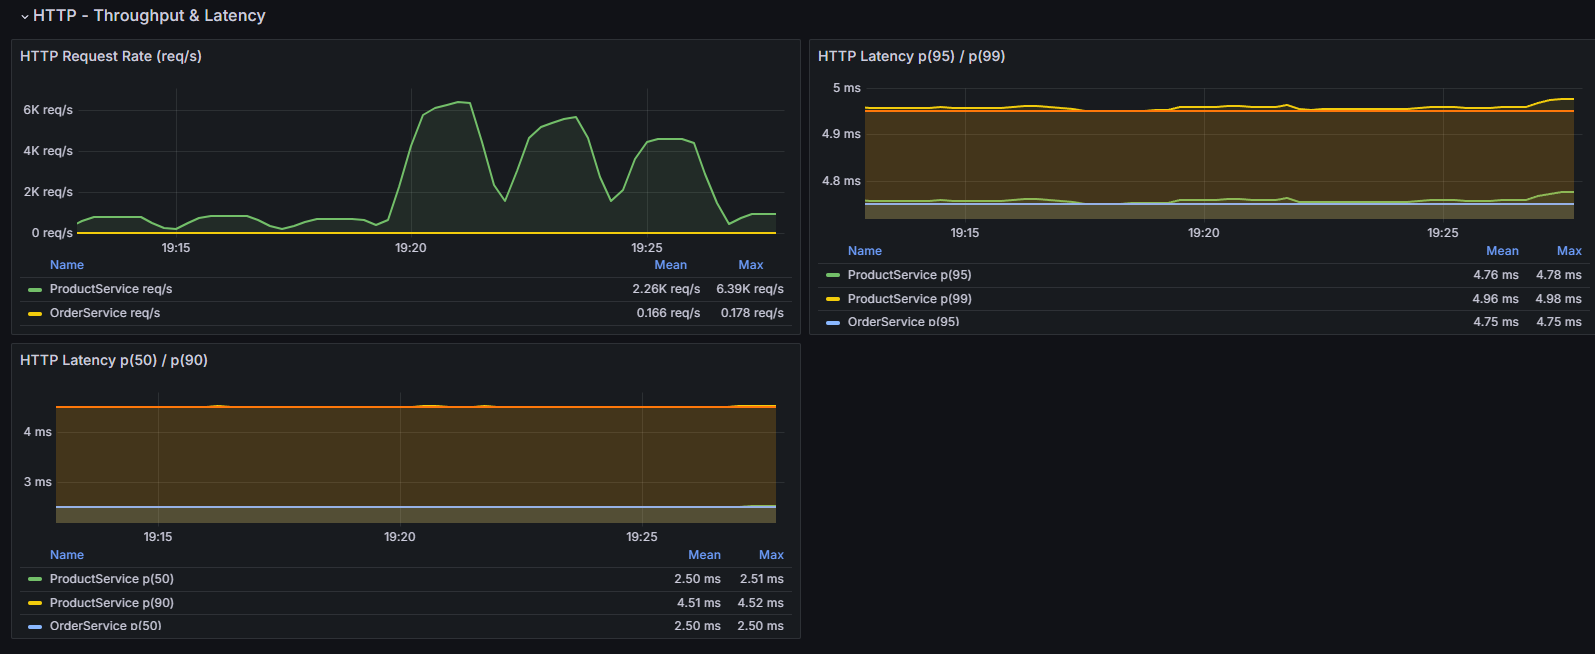
\includegraphics[width=\textwidth]{figures/grafana-1.png}
\caption{Pulpit Grafany -- liczba żądań na~sekundę oraz percentyle czasu obsługi żądania po~stronie usług \texttt{ProductService} i~\texttt{OrderService}}
\label{fig:GrafanaHttp}
\end{figure}

\begin{figure}[htb]
\centering
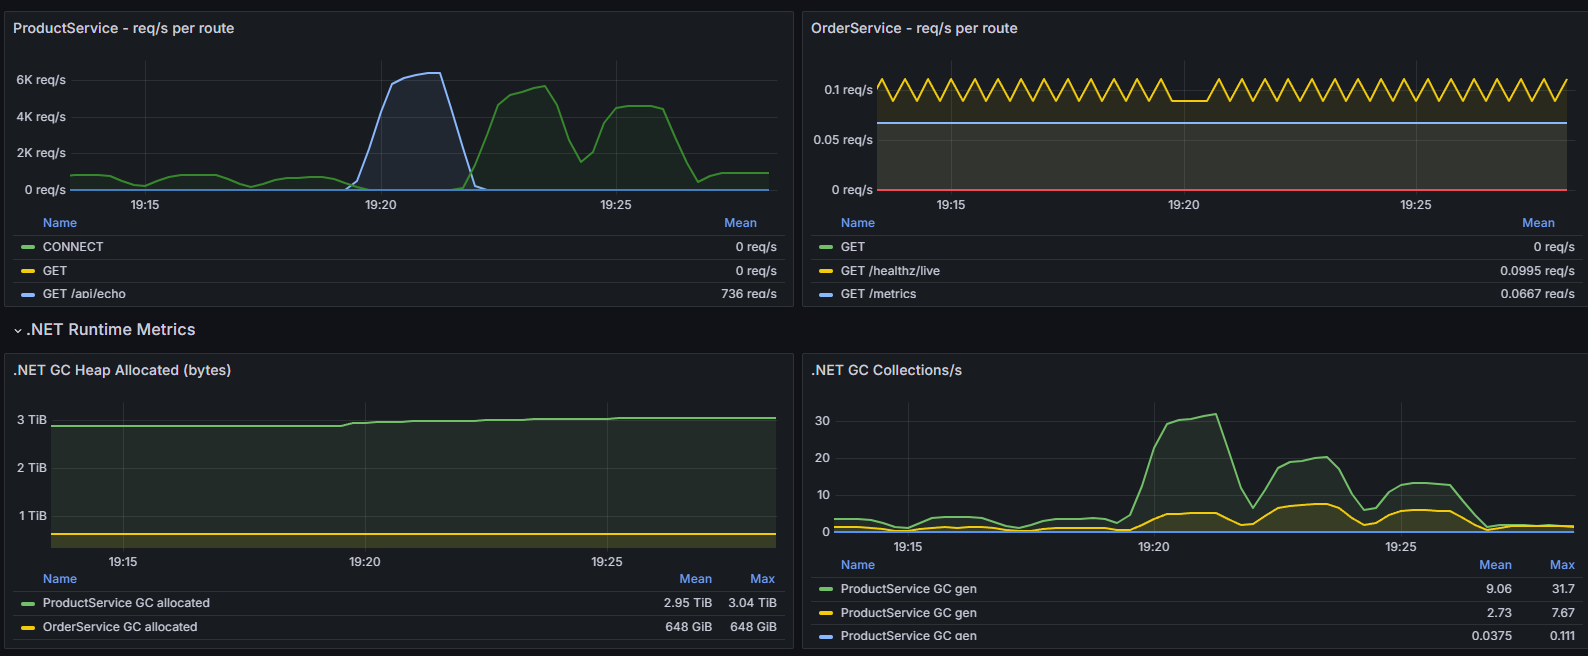
\includegraphics[width=\textwidth]{figures/grafana-2.png}
\caption{Pulpit Grafany -- liczba żądań w~podziale na~trasy oraz metryki środowiska uruchomieniowego .NET: wolumen alokacji i~częstość odśmiecania pamięci}
\label{fig:GrafanaRuntime}
\end{figure}

Zestawienie obu pulpitów ilustruje różnicę pomiędzy pomiarem serwerowym a~pomiarem po~stronie klienta. Czas obsługi żądania rejestrowany przez usługę wyrażony jest w~pojedynczych milisekundach, natomiast czas mierzony w~przeglądarce -- w~dziesiątkach milisekund. Rozbieżność ta~nie jest sprzecznością: metryka serwerowa obejmuje wyłącznie przetwarzanie żądania wewnątrz procesu usługi, natomiast pomiar kliencki -- pełną ścieżkę wraz z~propagacją sieciową, transmisją ładunku, deserializacją w~silniku JavaScript oraz aktualizacją drzewa dokumentu. Zestawienie obu wielkości wskazuje zatem, że~udział samego przetwarzania serwerowego w~czasie odczuwanym przez użytkownika pozostaje w~badanym systemie niewielki, co~stanowi niezależne potwierdzenie wniosku sformułowanego w~rozdziale~\ref{cha:AnalizaWydajnosci}.

Przedstawione przebiegi zarejestrowano w~trakcie obciążeniowej weryfikacji stosu obserwowalności, nie zaś podczas przebiegu macierzy badawczej. Wartości liczbowe widoczne na~panelach nie są~zatem porównywalne z~wynikami z~rozdziału~\ref{cha:AnalizaWydajnosci}; ilustrują one działanie warstwy monitorowania, a~nie rezultaty eksperymentu.

Listing~\ref{lst:OtelDotNet} przedstawia konfigurację śledzenia w~\texttt{OrderService}, wskazującą bezpośrednio na~punkt końcowy kolektora wykorzystany w~eksperymencie.

\begin{lstlisting}[
  language={[Sharp]C},
  breaklines=true,
  caption={Konfiguracja śledzenia OpenTelemetry w~OrderService z~eksportem do~Jaegera},
  label=lst:OtelDotNet
]
builder.Services.AddOpenTelemetry()
    .WithTracing(tracing => tracing
        .AddAspNetCoreInstrumentation()
        .AddEntityFrameworkCoreInstrumentation()
        .AddSource("MassTransit")
        .AddOtlpExporter(opt =>
        {
            // Jaeger collector inside the Docker network
            opt.Endpoint = new Uri("http://jaeger:4317");
        }));
\end{lstlisting}

Instrumentacja obejmuje trzy warstwy: obsługę żądań w~ASP.NET Core, zapytania Entity Framework Core oraz przepływ komunikatów w~MassTransit. Dzięki temu Jaeger umożliwia wizualizację pełnego łańcucha przyczynowo-skutkowego: od~żądania tworzącego zamówienie, poprzez zapis w~bazie wraz z~komunikatem Outbox, dostarczenie komunikatu do~brokera, aż~po~obsłużenie zdarzenia przez maszynę stanów. Zdolność diagnostyczna tego rodzaju jest szczególnie wartościowa w~architekturze mikroserwisowej, w~której tradycyjne debugowanie krokowe jest niewykonalne~\cite{bib:Nygard2018}.

Warstwa obserwowalności pełniła w~eksperymencie funkcję pomocniczą, nie pomiarową. Wartości przedstawione w~rozdziale~\ref{cha:AnalizaWydajnosci} pochodzą z~pomiaru wykonywanego po~stronie klienta, natomiast metryki i~ślady służyły weryfikacji, czy zachowanie systemu odpowiada oczekiwaniom -- w~szczególności czy trafienia w~pamięć podręczną występują tam, gdzie zakładano, oraz czy przepływ zdarzeń asynchronicznych rzeczywiście zachodzi.

% -----------------------------------------------------------------------
\subsection{Automatyzacja budowania}
\label{subsec:CI}
% -----------------------------------------------------------------------

Realizacja zasady niezależnego wdrażania usług wymaga automatyzacji budowania i~weryfikacji kodu. Fundamentem metodologicznym pozostaje tu~metodyka \textit{Twelve-Factor App}~\cite{bib:WigginsFactors}, zgodnie z~którą każda usługa powinna być budowana przez dedykowany potok i~wdrażana niezależnie od~pozostałych komponentów.

W~projekcie zdefiniowano potok \textit{GitHub Actions} uruchamiany po~zatwierdzeniu zmian w~gałęziach \texttt{main} i~\texttt{develop} oraz przy zgłoszeniu żądania scalenia. Potok podzielono na~trzy zadania: kompilację backendu, kompilację aplikacji frontendowej oraz budowanie obrazów kontenerów. Listing~\ref{lst:GithubActions} przedstawia jego strukturę w~postaci skróconej.

\begin{lstlisting}[
  language={},
  caption={Struktura potoku budowania w~GitHub Actions (fragment)},
  label=lst:GithubActions
]
name: CI
on:
  push:
    branches: [main, develop]
  pull_request:
    branches: [main]

jobs:
  backend:
    runs-on: ubuntu-latest
    steps:
      - uses: actions/checkout@v4
      - uses: actions/setup-dotnet@v4
        with: { dotnet-version: '10.0.x' }
      - run: dotnet build architecture-microservices-technical.sln
             --configuration Release

  frontend:
    runs-on: ubuntu-latest
    defaults:
      run: { working-directory: frontend/angular-app }
    steps:
      - uses: actions/checkout@v4
      - uses: actions/setup-node@v4
        with: { node-version: '20', cache: npm }
      - run: npm ci
      - run: npm run build -- --configuration production

  docker:
    runs-on: ubuntu-latest
    needs: [backend]
    steps:
      - uses: actions/checkout@v4
      - uses: docker/setup-buildx-action@v3
      - uses: docker/build-push-action@v5
        with:
          file: backend/ProductService/Dockerfile
          push: false
          cache-from: type=gha
          cache-to: type=gha,mode=max
\end{lstlisting}

Budowanie obrazów uzależniono od~powodzenia kompilacji backendu, co~zapobiega tworzeniu obrazów z~kodu, który się nie kompiluje. Zadania backendu i~frontendu wykonują się równolegle, ponieważ nie zachodzi między nimi zależność, a~pamięć podręczna warstw przechowywana w~infrastrukturze GitHub skraca czas kolejnych przebiegów.

Należy przy tym precyzyjnie określić zakres tej automatyzacji. Potok weryfikuje wyłącznie \textbf{poprawność kompilacji} obu mikroserwisów, aplikacji frontendowej oraz budowania obrazów kontenerów. Nie uruchamia testów automatycznych, nie publikuje obrazów do~rejestru ani nie realizuje wdrożenia. Jest to~zatem potok ciągłej integracji, a~nie ciągłego dostarczania; samo wdrożenie na~serwer wykonywano w~sposób opisany w~sekcji~\ref{subsec:Deployment}. Rozszerzenie potoku o~testy integracyjne oraz automatyczne wdrożenie wskazano jako kierunek dalszego rozwoju.

% -----------------------------------------------------------------------
\section{Konsekwencje wyników dla decyzji wdrożeniowych}
\label{sec:WnioskiWdrozeniowe}
% -----------------------------------------------------------------------

Rekomendacje przedstawione w~sekcji~\ref{sec:Rekomendacje} dotyczą wyboru protokołu komunikacji. Zmierzone zależności prowadzą jednak również do~wniosków odnoszących się do~infrastruktury, w~której system jest wdrażany, i~te~omówiono poniżej. Ich wspólną podstawą jest ustalenie, że~w~badanym zakresie czas odpowiedzi wyznaczany jest przez liczbę wymian pakietów oraz opóźnienie łącza, nie przez wydajność przetwarzania po~stronie serwera.

\begin{enumerate}
\item \textbf{Rozmieszczenie geograficzne przed wyborem protokołu.} Skoro przewaga serializacji binarnej wyraża się liczbą zaoszczędzonych obiegów pakietu, a~koszt każdego z~nich jest proporcjonalny do~opóźnienia łącza, to~skrócenie samego opóźnienia oddziałuje na~ten~sam składnik czasu odpowiedzi, przy czym korzyść ta~występuje w~całym zakresie rozmiarów odpowiedzi, także poniżej rozmiaru okna odbiorczego. Wybór regionu centrum danych oraz ewentualne zakończenie połączenia w~punkcie obecności bliższym użytkownikowi stanowią zatem dźwignię działającą szerzej niż zmiana protokołu, która pozostaje bezskuteczna poniżej rozmiaru okna odbiorczego. Decyzję o~rozmieszczeniu należy w~konsekwencji podejmować przed decyzją o~protokole, nie po~niej.

\item \textbf{Skalowanie nie usuwa ograniczenia leżącego w~sieci.} W~trakcie pomiarów wykorzystanie procesora serwera nie przekroczyło 250\% wobec 800\% dostępnych, a~przepustowość dysku pozostała poniżej 800~KB/s (sekcja~\ref{subsec:SrodowiskoUruchomieniowe}), natomiast czynnik ograniczający zidentyfikowano po~stronie stanowiska klienckiego (sekcja~\ref{sec:GranicaNarzedzia}). Ani powiększenie instancji, ani zwielokrotnienie replik usług nie zmieniłoby w~tych warunkach zmierzonych czasów odpowiedzi. Wniosek ten jest przeciwny do~odruchu typowego przy problemach wydajnościowych i~wskazuje, że~przed podjęciem decyzji o~skalowaniu konieczne jest ustalenie, po~której stronie znajduje się wąskie gardło.

\item \textbf{Kompresja jako punkt konfiguracyjny infrastruktury.} Kompresja ciała odpowiedzi bywa włączana nie w~usłudze, lecz w~odwrotnym proxy, w~sieci dostarczania treści albo w~warstwie brzegowej, a~zatem poza kodem aplikacji. Jak wykazano w~sekcji~\ref{subsec:Kompresja}, jej zastosowanie sprowadza wszystkie badane ładunki poniżej rozmiaru jednego okna odbiorczego, znosząc mechanizm odpowiadający za~zmierzoną przewagę. Konfiguracja warstwy brzegowej rozstrzyga więc o~tym, czy zmiana protokołu przyniesie jakikolwiek efekt, co~czyni ją~decyzją poprzedzającą, a~nie towarzyszącą.

\item \textbf{Asymetria kosztów obu dźwigni.} Zmiana protokołu komunikacji obciąża budżet jednorazowym kosztem prac inżynierskich, nie zwiększając kosztu bieżącego, natomiast zmiana rozmieszczenia lub rozmiaru infrastruktury podnosi rachunek okresowy na~stałe. Porównanie obu ścieżek ma~zatem sens dopiero po~ustaleniu, czy typowa odpowiedź systemu przekracza rozmiar okna odbiorczego, ponieważ poniżej tego progu pierwsza z~nich nie przynosi efektu, a~druga pozostaje jedyną skuteczną.
\end{enumerate}

Zestawienie to~wskazuje, że~wynik pracy ma~znaczenie nie tylko dla wyboru mechanizmu komunikacji, lecz także dla kolejności decyzji infrastrukturalnych: rozmieszczenie oraz konfiguracja warstwy brzegowej rozstrzygają o~tym, czy przestrzeń na~optymalizację protokołu w~ogóle istnieje.

% -----------------------------------------------------------------------
\section{Testowanie i~walidacja rozwiązań}
\label{sec:TestowanieWalidacja}
% -----------------------------------------------------------------------

Walidacja systemu eShop obejmuje poprawność funkcjonalną, wiarygodność wyników eksperymentalnych oraz zgodność zaobserwowanego zachowania systemu z~założeniami przyjętymi na~etapie projektowania.

\subsection{Walidacja wyników eksperymentu}
\label{subsec:WalidacjaWynikow}

Wiarygodność wyników przedstawionych w~rozdziale~\ref{cha:AnalizaWydajnosci} potwierdzona została następującymi mechanizmami kontrolnymi:

\begin{enumerate}
    \item \textbf{Pięciokrotne powtórzenie całej macierzy} -- każdą z~39~konfiguracji wykonano w~pięciu przebiegach z~rotowaną kolejnością protokołów, co~pozwoliło ocenić powtarzalność pomiarów oraz zweryfikować stałość kierunku relacji pomiędzy protokołami, nie tylko ich uśrednione wartości.

    \item \textbf{Zerowy wskaźnik błędów} -- w~585~wykonanych testach i~171~tysiącach pomiarów nie zarejestrowano ani jednego żądania zakończonego niepowodzeniem. Potwierdza to, że~zmierzone wartości opisują poprawnie zrealizowane wywołania.

    \item \textbf{Weryfikacja modelu na~danych niezależnych} -- model liczby wymian pakietów (sekcja~\ref{sec:ModelOkna}), wyprowadzony z~pomiaru charakterystyki łącza, przewiduje zmierzone czasy odpowiedzi w~dziesięciu konfiguracjach z~dokładnością do~0,2~obiegu pakietu. Zgodność ta~jest szczególnie mocną przesłanką, ponieważ model opiera się na~parametrach wyznaczonych niezależnie od~samych pomiarów opóźnień.

    \item \textbf{Rozdzielenie czynników przez grupę kontrolną} -- wariant z~proxy Envoy, przenoszący ładunek binarny po~protokole HTTP/1.1, umożliwił oddzielenie wpływu formatu serializacji od~wpływu wersji protokołu HTTP (sekcja~\ref{sec:Dekompozycja}). Bez tej grupy kontrolnej oba czynniki pozostałyby zmieszane.

    \item \textbf{Pomiarowa weryfikacja założeń} -- rozmiary odpowiedzi, parametry łącza oraz negocjowana wersja protokołu HTTP zostały zmierzone, nie przyjęte na~podstawie dokumentacji. W~jednym przypadku pomiar obalił wcześniejsze oszacowanie: przepustowość wyznaczona z~nachylenia zależności czasu odpowiedzi od~rozmiaru okazała się zawyżona o~rząd wielkości względem wartości zmierzonej bezpośrednio, ponieważ opierała się na~różnicy mieszczącej się w~granicach szumu.

    \item \textbf{Jawna polityka odrzucania obserwacji odstających} -- próbki przekraczające jedną sekundę wyłączono ze~statystyk zbiorczych na~podstawie udokumentowanej analizy diagnostycznej, przy zachowaniu w~wynikach zarówno ich liczby, jak i~kompletu statystyk wyznaczonych bez odrzucania (sekcja~\ref{subsec:PolitykaZaciec}).

    \item \textbf{Ustalenie umiejscowienia wąskiego gardła} -- odrębny pomiar skalowania (sekcja~\ref{sec:GranicaNarzedzia}) pozwolił ustalić, że~przy liczbie klientów przekraczającej dwadzieścia czynnik ograniczający znajduje się po~stronie stanowiska pomiarowego, i~ograniczyć macierz badawczą do~zakresu, w~którym pomiar pozostaje wiarygodny.

    \item \textbf{Ocena rozstrzygalności różnic} -- dla konfiguracji stanowiących podstawę wniosków wyznaczono przedziały ufności różnic sparowanych w~obrębie przebiegu (sekcja~\ref{sec:PrzedzialyUfnosci}), co~zastąpiło regułę opartą na~progu procentowym kryterium wiążącym ocenę ze~zmiennością danych. Rozstrzygalność każdej z~raportowanych różnic jest w~konsekwencji podana jawnie.

    \item \textbf{Sprawdzenie odporności na~wybór miary} -- wnioski powtórzono dla percentyla~95, wykazując, że~kierunek i~rząd wielkości relacji pomiędzy protokołami nie zależą od~przyjęcia mediany jako miary podstawowej (sekcja~\ref{subsec:OdpornoscMiary}).
\end{enumerate}

\subsection{Integracja wzorców z~wynikami wydajnościowymi}
\label{subsec:IntegracjaWzorcow}

Zestawienie wyników eksperymentu z~zaimplementowanymi wzorcami prowadzi do~wniosków przedstawionych w~tabeli~\ref{tab:PatternsImpact}.

\begin{table}[htb]
\centering
\footnotesize
\caption{Wpływ wzorców projektowych na~wydajność -- wnioski z~eksperymentu}
\label{tab:PatternsImpact}
\begin{tabular}{|p{3.2cm}|p{4.5cm}|p{4.5cm}|}
\hline
\textbf{Wzorzec} & \textbf{Korzyść wydajnościowa} & \textbf{Koszt wydajnościowy} \\
\hline
Cache-Aside (Redis) & Skrócenie czasu odpowiedzi oraz obniżenie zmienności wyniku o~rząd wielkości & Konieczność unieważniania wpisów przy zmianie kształtu odpowiedzi \\
\hline
Transactional Outbox & Gwarancja dostarczenia zdarzeń bez dwufazowego zatwierdzania transakcji & Składnik stały rzędu 60--70\,ms w~operacjach zapisu \\
\hline
Saga (MassTransit) & Orkiestracja procesów bez blokujących wywołań synchronicznych; w~zrealizowanym systemie wykorzystana w~zakresie utworzenia instancji procesu & Koszt utrwalenia stanu instancji w~bazie danych, wliczony w~pomiar operacji zapisu \\
\hline
Serializacja binarna & Redukcja wolumenu danych o~42--43\%, przekładająca się na~26--43\% czasu odpowiedzi przy dużych ładunkach & Koszt deserializacji w~silniku JavaScript; brak korzyści przy ładunkach mieszczących się w~jednym oknie \\
\hline
Pula kontekstów bazodanowych & Eliminacja tworzenia kontekstu EF~Core przy każdym żądaniu & Wymóg braku stanu przenoszonego pomiędzy żądaniami w~obiekcie kontekstu \\
\hline
\end{tabular}
\end{table}

Zestawienie scenariuszy Orders i~Echo pozwala oszacować łączny koszt warstwy persystencji wraz z~wzorcem Outbox. Utworzenie zamówienia z~dziesięcioma pozycjami zajmuje około 94~ms, natomiast żądanie do~punktu końcowego nieodwołującego się do~bazy danych -- około 32~ms przy porównywalnym rozmiarze odpowiedzi. Różnica rzędu 60~ms obejmuje walidację, zapis encji zamówienia i~jego pozycji, atomowy zapis komunikatu Outbox oraz zatwierdzenie transakcji.

Szacunek ten należy traktować jako przybliżony, ponieważ zestawiane scenariusze różnią się nie tylko obecnością warstwy persystencji, lecz także kierunkiem przesyłanych danych: scenariusz Echo zwraca kolekcję rekordów, natomiast scenariusz zapisu przyjmuje treść żądania i~zwraca potwierdzenie utworzenia zasobu. Uzyskana wartość wskazuje zatem rząd wielkości kosztu operacji zapisu, nie jego dokładną miarę.

Jest to~świadomy kompromis architektoniczny. Gwarancja atomowości zapisu danych biznesowych oraz komunikatu zdarzenia eliminuje klasę błędów polegających na~utracie zdarzeń przy awarii występującej pomiędzy zatwierdzeniem transakcji a~publikacją komunikatu. Rozwiązanie alternatywne w~postaci dwufazowego zatwierdzania transakcji wprowadziłoby wyższy narzut oraz zależność od~dostępności koordynatora transakcji~\cite{bib:Richardson2018}.

Studium przypadku systemu eShop potwierdza, że~wzorce omówione w~części teoretycznej pracy mogą być skutecznie zaimplementowane w~ekosystemie .NET~10 z~akceptowalnym narzutem wydajnościowym. Wniosek nadrzędny jest jednak inny i~wykracza poza katalog wzorców: charakterystyka wydajnościowa systemu rozproszonego wyznaczana jest przede wszystkim przez właściwości warstwy, która w~danym scenariuszu stanowi wąskie gardło. W~operacjach zapisu jest to~warstwa persystencji wraz z~wzorcami zapewniającymi spójność, w~odczycie dużych zbiorów danych -- liczba wymian pakietów wynikająca z~wolumenu odpowiedzi, w~odczycie małych ładunków -- opóźnienie propagacji sieciowej. Wybór protokołu komunikacji wpływa wyłącznie na~drugi z~tych przypadków, co~powinno wyznaczać zarówno kolejność działań optymalizacyjnych, jak i~oczekiwania wobec ich rezultatów.
